\begin{apendicesenv}
\partapendices

\chapter{Cronograma Detalhado}
\label{schedule_ap}

Para evitar poluição visual no relatório, foram feitas duas versões do cronograma.
Dentro do relatório foi incluída uma versão simplificado do mesmo, sem o detalhamento de todas as atividades.
As figuras seguintes mostram o cronograma detalhado.

\begin{figure}[!htbp]
  \centering
  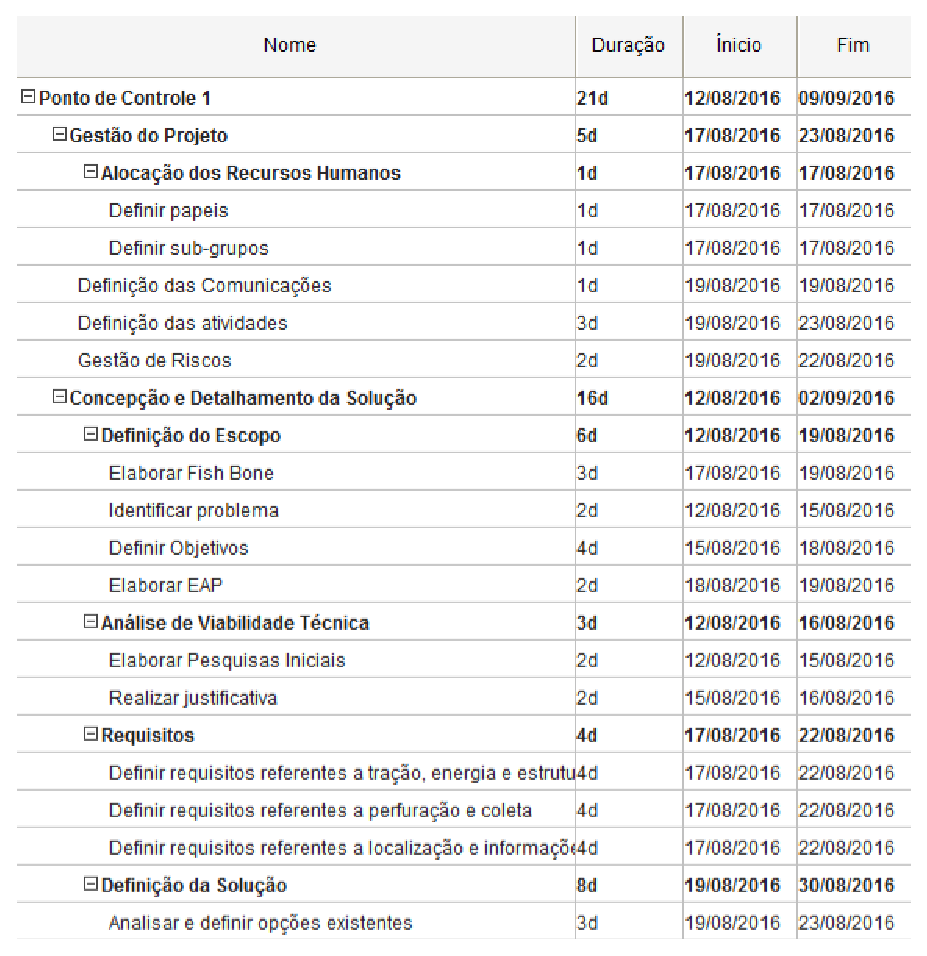
\includegraphics[width=\textwidth]{figuras/cronograma_det_1.eps}
  \caption{Cronograma de Atividades detalhado (parte 1). Fonte: autores.}
  \label{fig:cron_d1}
\end{figure}

\vfill
\pagebreak

\begin{figure}[!htbp]
  \centering
  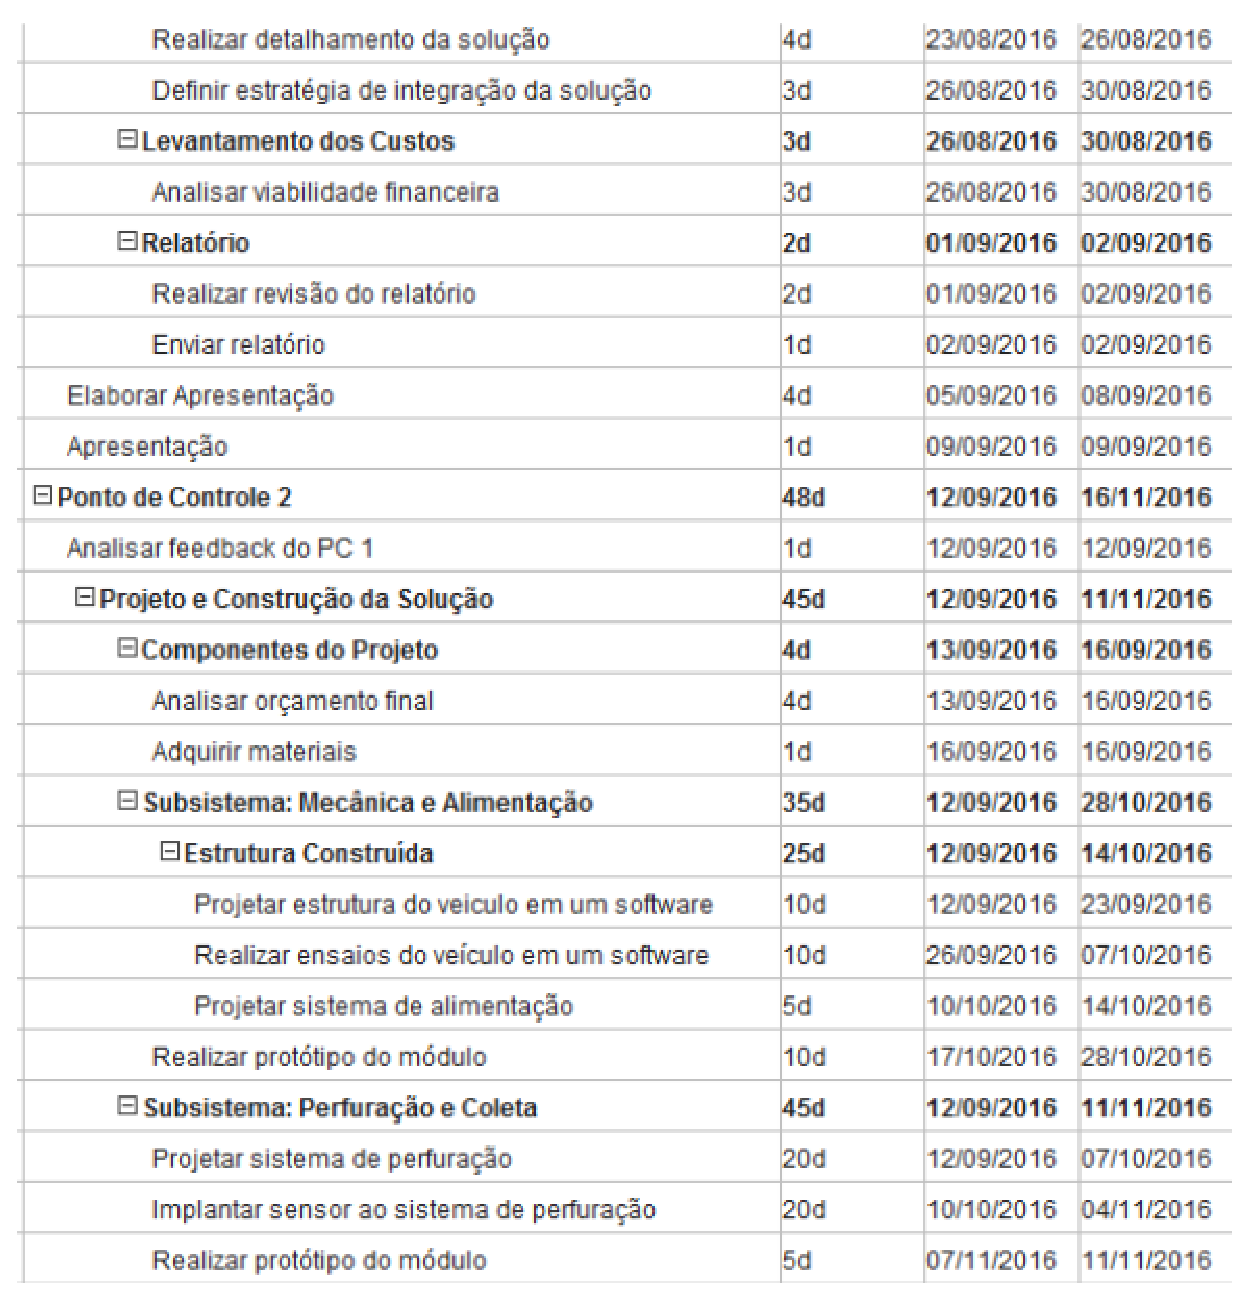
\includegraphics[width=\textwidth]{figuras/cronograma_det_2.eps}
  \caption{Cronograma de Atividades detalhado (parte 2). Fonte: autores.}
  \label{fig:cron_d2}
\end{figure}

\vfill
\pagebreak

\begin{figure}[!htbp]
  \centering
  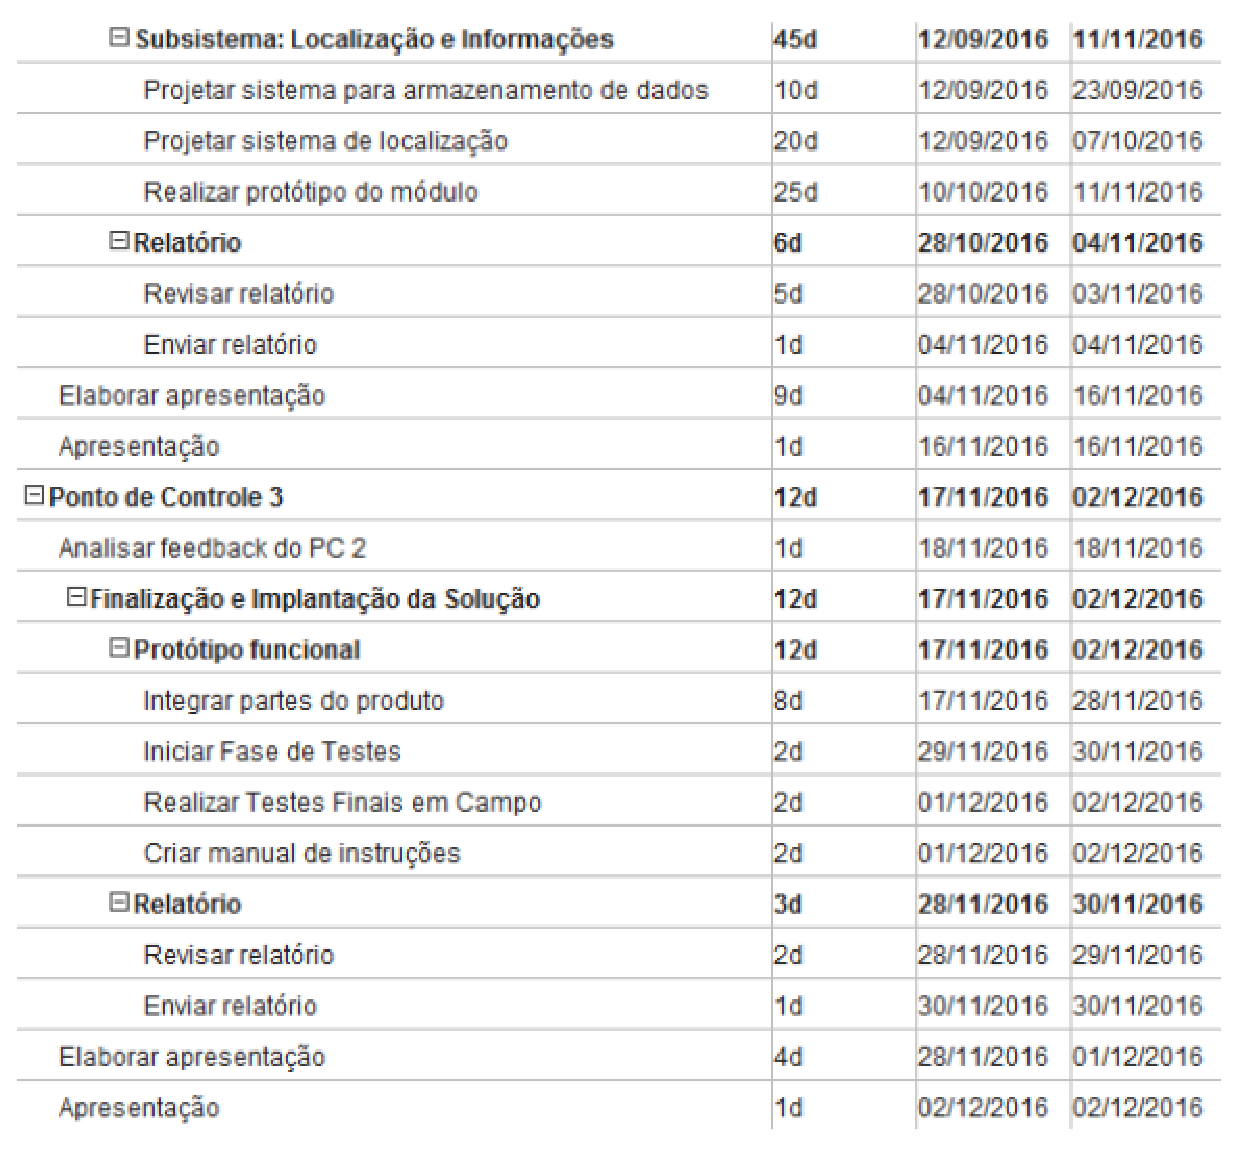
\includegraphics[width=\textwidth]{figuras/cronograma_det_3.eps}
  \caption{Cronograma de Atividades detalhado (parte 3). Fonte: autores.}
  \label{fig:cron_d3}
\end{figure}

\chapter{Desenhos Técnicos da Estrutura}

\begin{figure}[!htbp]
	\centering
	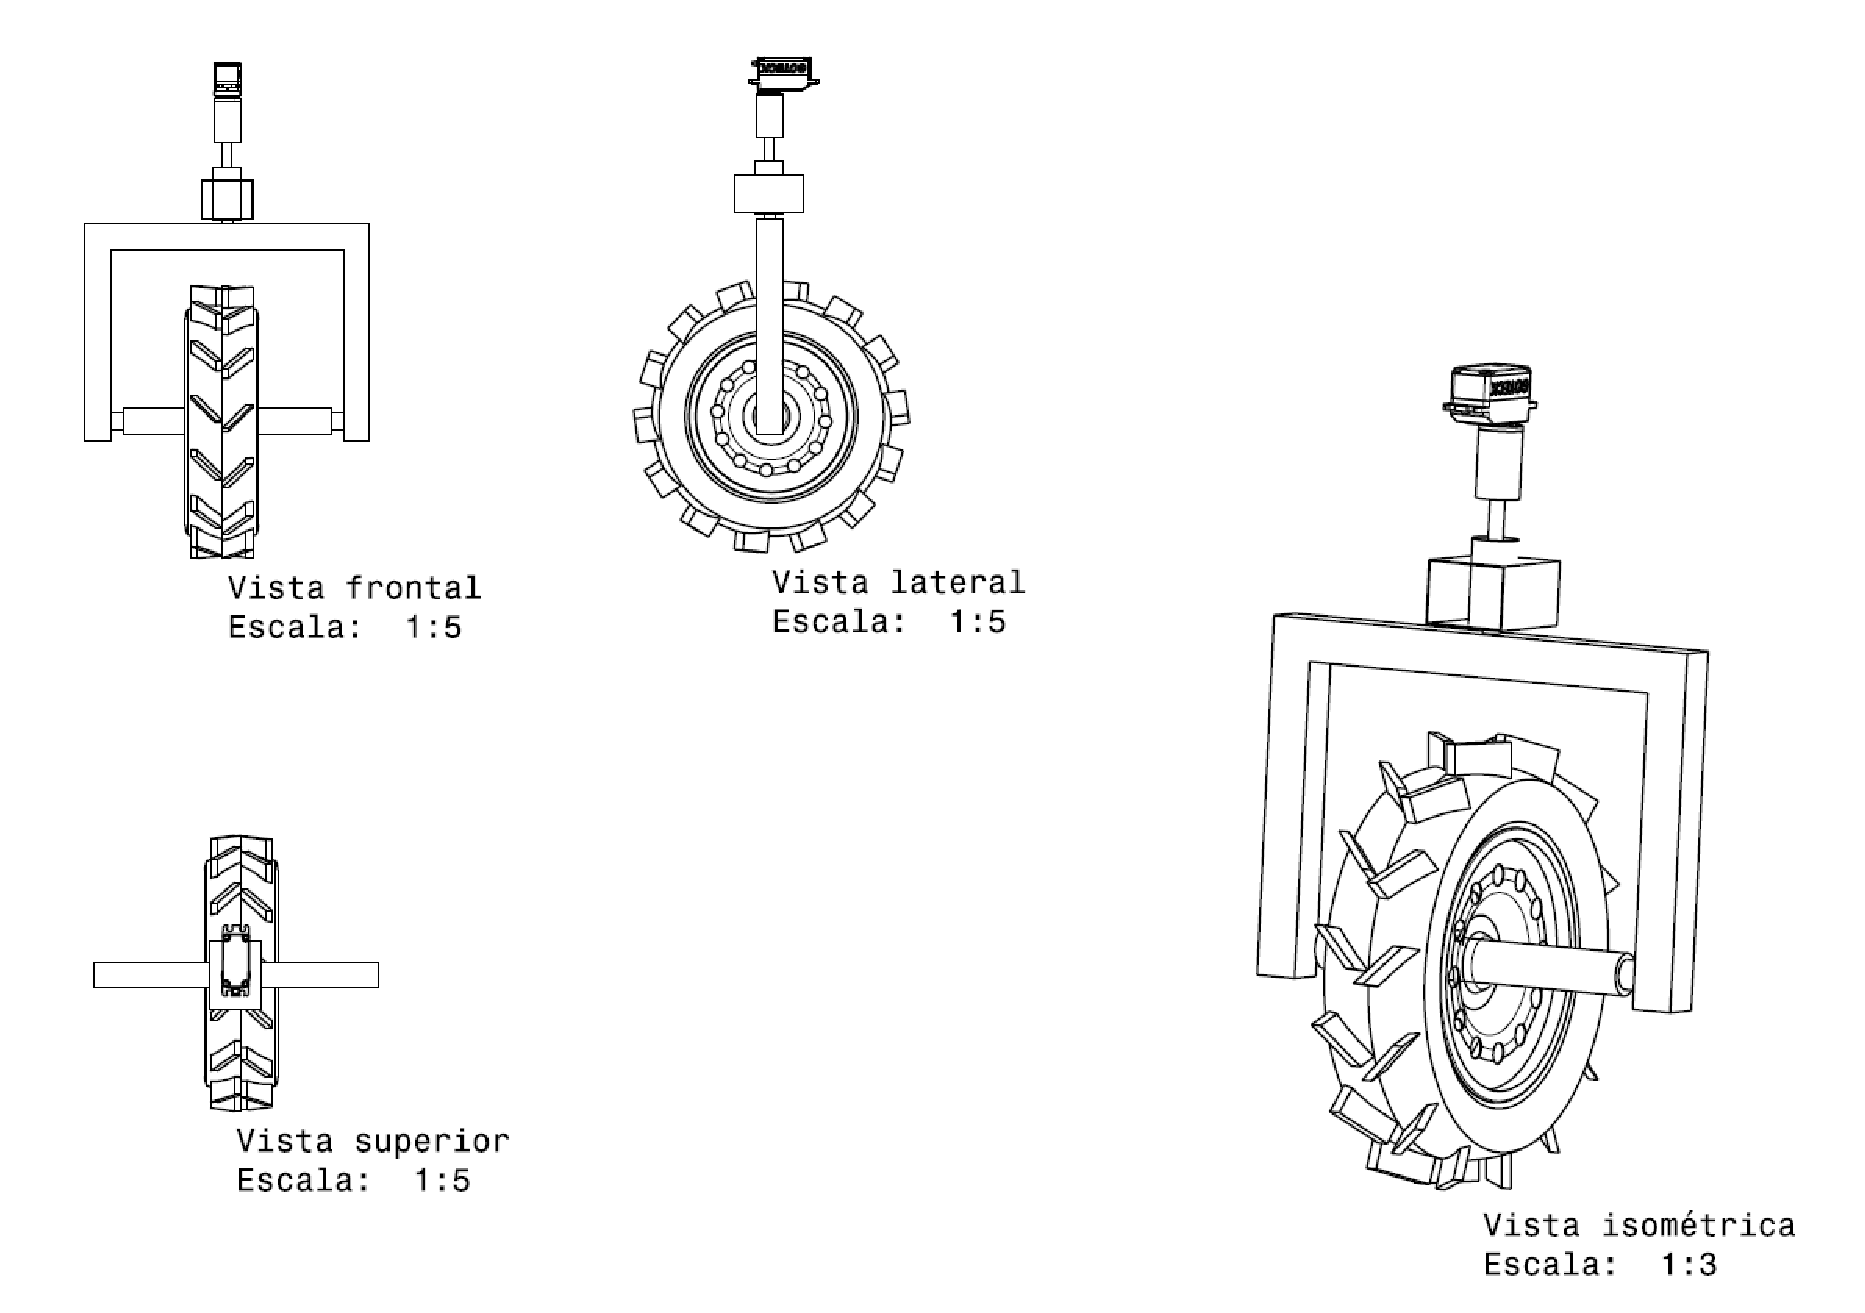
\includegraphics[width=\textwidth]{figuras/dt_direcao1.eps}
	\caption{Vistas frontal, lateral e superior da estrutura da direção}
\end{figure}

\begin{figure}[!htbp]
	\centering
	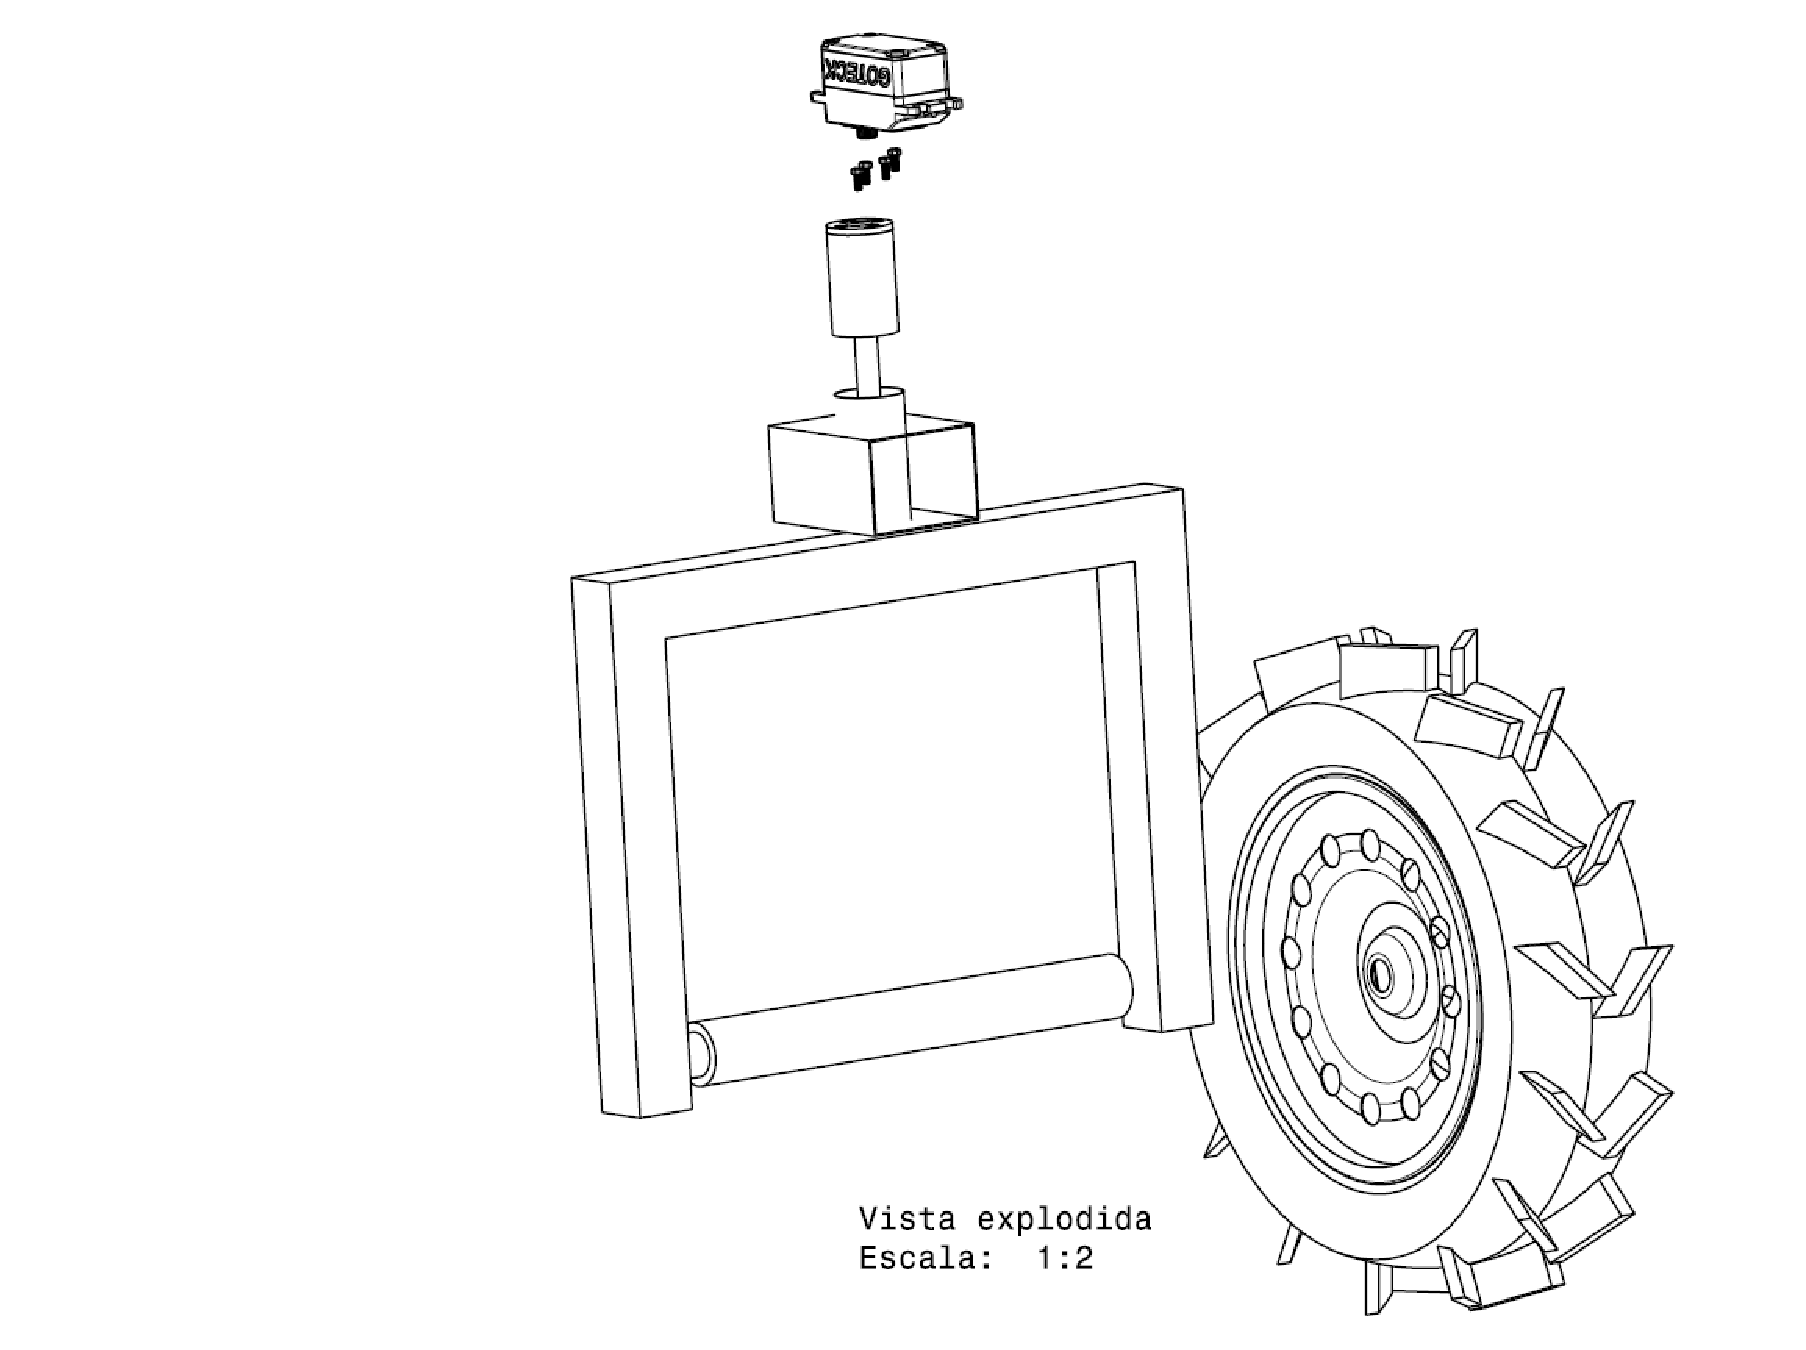
\includegraphics[width=\textwidth]{figuras/dt_direcao2.eps}
	\caption{Vista explodida do sistema de direção}
\end{figure}

\begin{figure}[!htbp]
	\centering
	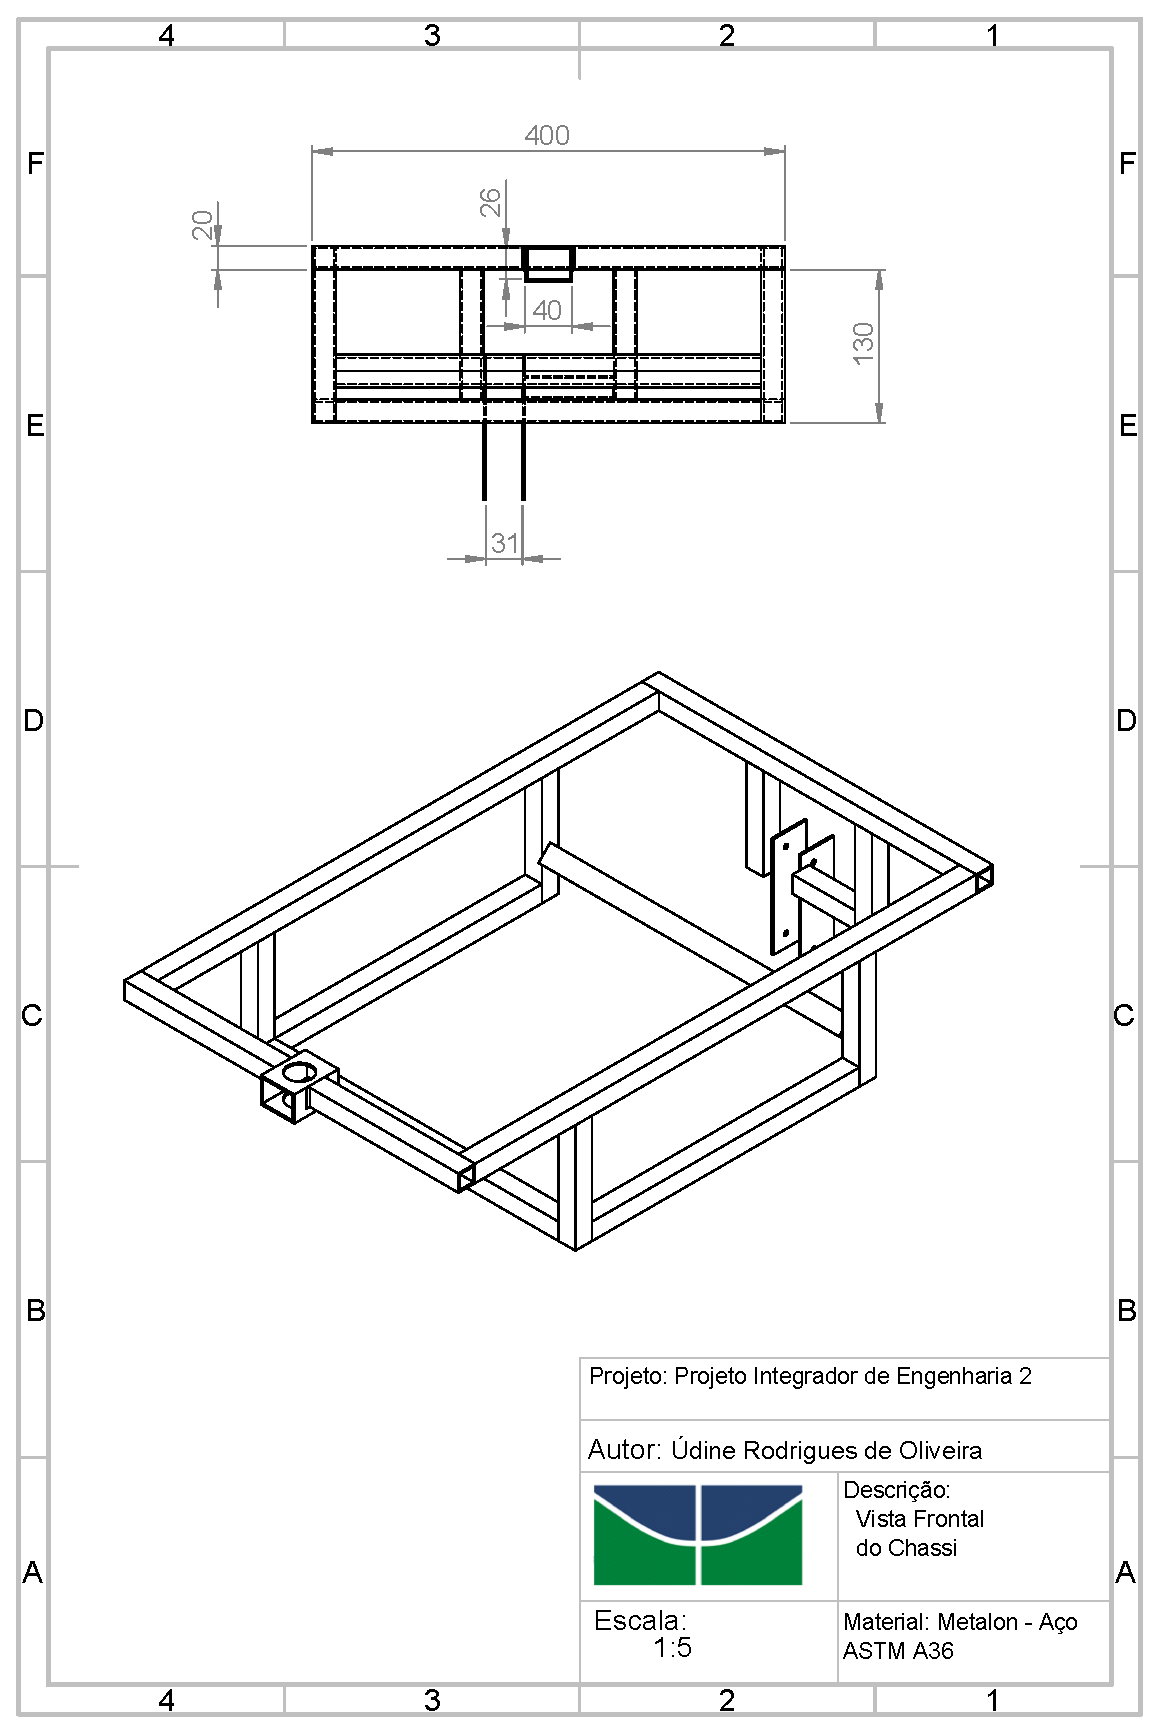
\includegraphics[width=\textwidth]{figuras/chassi_frontal.eps}
	\caption{Desenho técnico da vista frontal do chassi}
\end{figure}

\begin{figure}[!htbp]
	\centering
	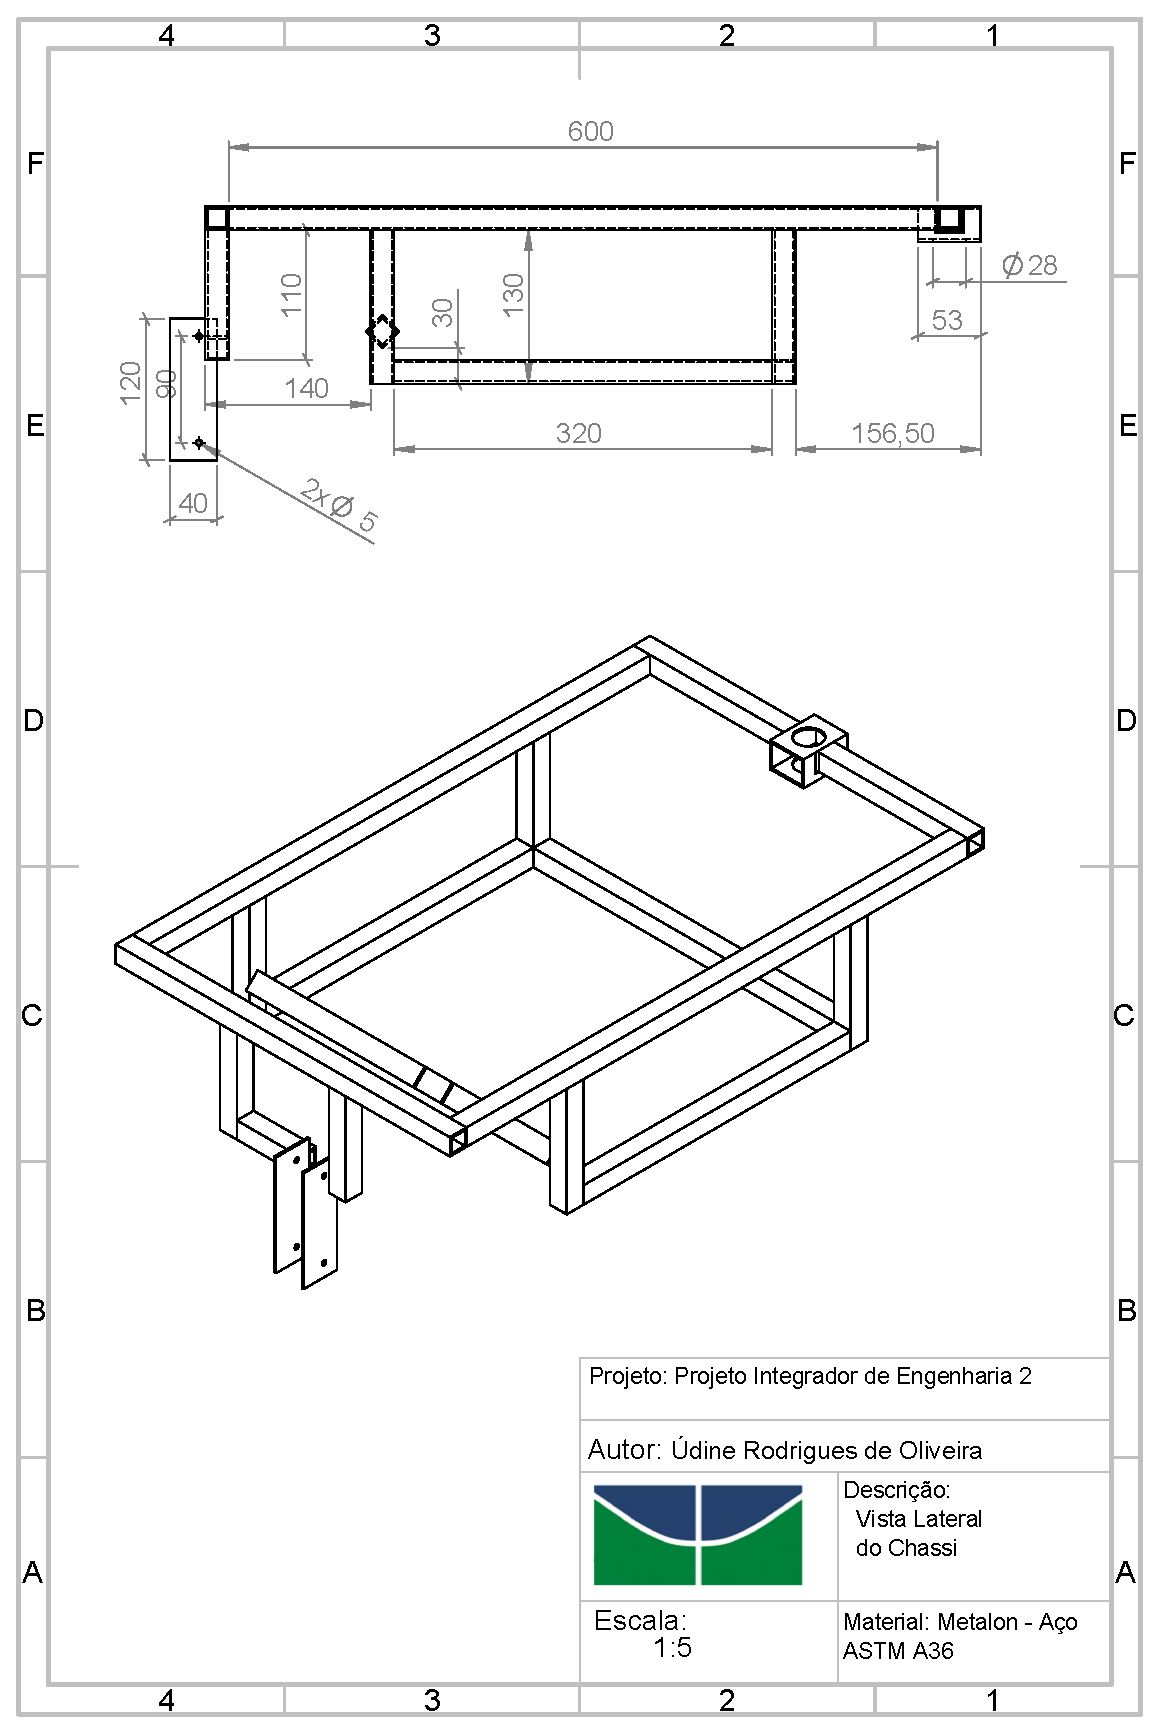
\includegraphics[width=\textwidth]{figuras/chassi_lateral.eps}
	\caption{Desenho técnico da lateral frontal do chassi}
\end{figure}

\begin{figure}[!htbp]
	\centering
	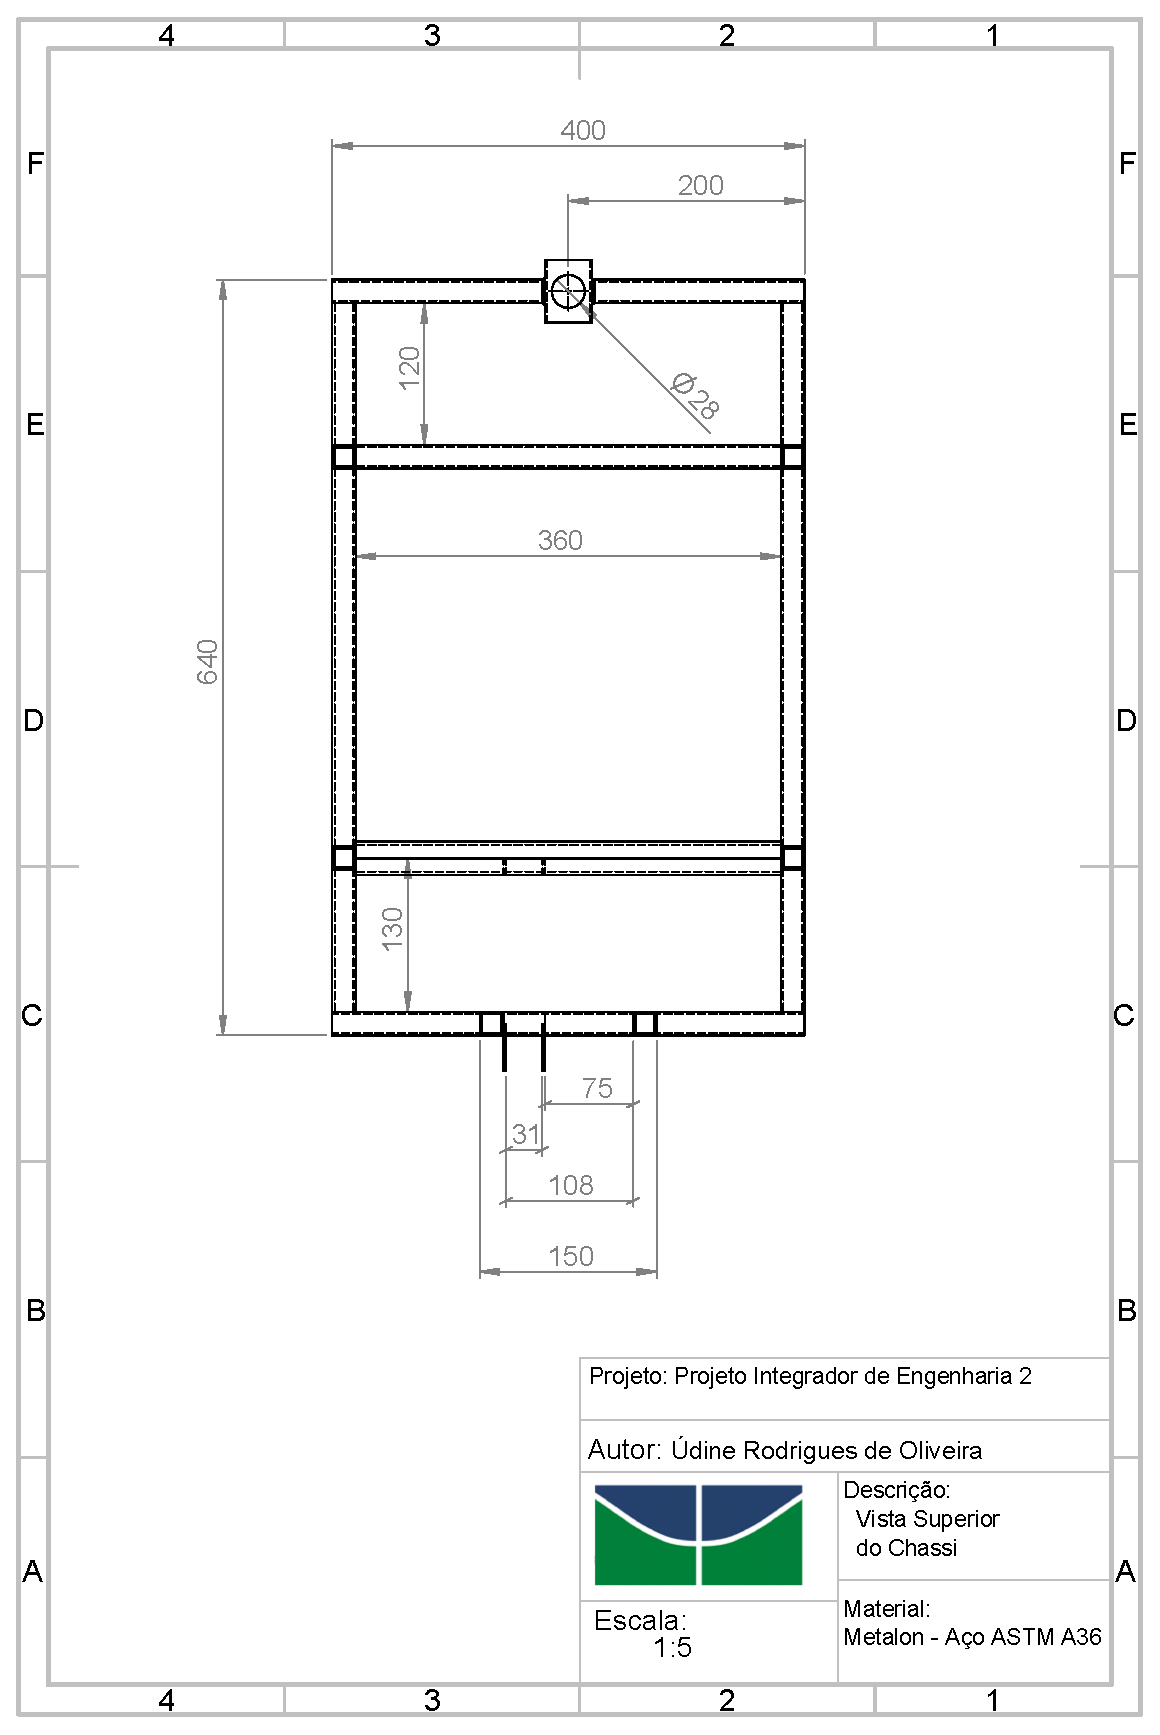
\includegraphics[width=\textwidth]{figuras/chassi_superior.eps}
	\caption{Desenho técnico da vista superior do chassi}
\end{figure}

\chapter{Manual de instruções}
\label{manuel}

Esse sistema é para a gerência do estado de sua plantação e configuação do carro autônomo para monitoramento de sua plantação de morango.

Ao acessar o sistema você irá se deparar com a página inicial onde terá quatro opções e uma ação, sendo que uma das quatro opções é o
manual que aqui se encontra.

\subsection{Configurações Gerais}

A primeira opção "Configurações Gerais", você irá se deparar com a opção de baixar os dados para que você obtenha as informações
coletadas pelo carro e também que você possa recuperar as medições feitas pelo veículo, se de alguma forma ocorrer perca dos dados
do seu sistema, com essa opção você recuperar esses dados do carro autônomo.

A outra opção você deverá antes de colocar o carro para trabalhar monitorando o campo, incluir as informações relacionado a quantidade
de fileiras ou cramalhões de sua plantação, para que o carro saiba quantas fileiras deve percorrer e quando deve ser sua parada.

A outra opção é relacionada a configuração de acesso ao carro autônomo, baseado nessa confoguração que ele consefuirá mandar os
dados que o mesmo precisa. A princípio essa opção já vem configurada, não precisando alterá-la, a não ser que você necessite
alterar o endereço de acesso ao carro.

\subsection{Minhas Medições}

A segunda opção "Minhas Medições" você poderá obter as informações coletadas pelo carro e com base neles, realizar a gerência
de sua plantação. Para que os dados apareçam, é necessário antes baixar as informações na opção de configurações gerais, e já
na opção Minha Medições, clicar no botão "Ler" para que o sistema leia os dados obtidos do carro e traga as informações.
Aqui você poderá verificar os dados principais que são umidade do solo, umidade do ar e temperatura do ar. Como observação a
umidade do solo ideal para plantações de morango deve estar entre 20 e 21 porcento.

\subsection{Calibração do sensor}

A terceira opção "Calibração do sensor" é onde você terá que antes de colocar o carro em ação para monitoração, calibrar
o sensor de umidade do solo do carro, pois caso não seja calibrado, os dados de umidade do seu solo, virão incorretas, e
isso pode acarretar prejuízo a sua plantação. Para calibração, será necessário seguir os seguintes passos:

\begin{itemize}
  \item Pegar uma amostra do seu solo com peso aproximado de 100 gramas.
  \item Fazer a secagem desta amostra com auxílio do microondas com potência entre 60 a 80 porcento.
  \item Esperar o tempo de 240 segundos ou 4 minutos exatos para estabilização da massa do solo.
  \item Pesar a amostra de solo seco e verificar se o mesmo está com 100 gramas.
  \item Caso dê um valor acima, retirar o excesso até atingir o valor de 100 gramas, caso não atinja esse valor, será necessário completar a amostra e repetir o processo de secagem.
  \item Pegar uma amostra de água destilada com peso de 5 gramas e umedecer a amostra.
  \item Misturar bem a amostra até obter uma amostra homogênea.
  \item Realizar a medição dessa amostra com o sensor de umidade e obter o valor.
  \item Os valores dos pesos do solo e da água passados são intencionais, pois com estes valoress, dará um valor de umidade de 5 porcento.
  \item O valor obtido da medida do sensor com o valor da umidade a 5 porcento indicará que para esta umidade o valor da medida do sensor é equivalente.
  \item Repetir esse procedimento para amostra de solo com 10, 15, 20, 25, 30, 40, 50 e 60 porcento, sendo estas porcentagens equivalentes ao valor do peso da água, e incluir esses valoes no sistema na parte de calibração do sistema.
\end{itemize}

\subsection{Iniciar Medições}

Esse botão você irá iniciar o carro depois de colocá-lo no ponto inicial para que realize as suas medições em sua plantação.



























\end{apendicesenv}
